\section{Results}
	Painting segmentation: 88.57 \% correct segmentation
	\todo{qualitative as well as quantitative}
	
	\todo{quantitative: graphs, tables, roc-curves, f1-scores, ...}
	
	\todo{qualititative: technisch, show where and why the method succeeds or fails, pictures of easy and difficulty cases}
	
	Because our method relies heavily on edge detection, there are cases where this could have a negative impact. In many cases, there is a shadow underneath the painting, as shown on figure \ref{fig:negative_case_shadow}.
	
	\begin{figure}
		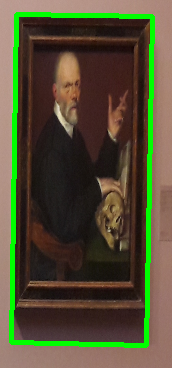
\includegraphics[width=\linewidth]{negative_case_shadow}
		\caption{An example of a shadow underneath the painting. This usually results in the segmentation algortihm to include this shadow as part of the painting because of the strong edge.}
		\label{fig:negative_case_shadow}
	\end{figure}